\documentclass{standalone}
\begin{document}
	\subsection{Lung Extraction}
	This is a pre processing step , which involves the creation of a lung mask and the managing of the Hounsfiel Unit. The creation of a mask for the lung regions, allow us to exclude the extra-lung regions from the segmentation, so reducing the number of clusters and avoiding the formation of false positives. In order to achieve this purpose, we have decided to use a pre-trained neural networks~\cite{REP:lungmask} which code is open source. We have decided to chose this pre-trained network since provide good results for the lung extraction. On the other hand, the use of a neural network avoid the problem that other kind of segmentation will have in presence of severe interstitial lung disease(ILD), that will be removed if method like threshold were applied, as we have see i the previous session.\\
	The used network is a U-Net,that is a modification of the convolutional neural network architecture useful for medical and biological field, because is developed to works also with a small training dataset\\
	The network provided 3 pre-trained models : 
	\begin{itemize}
		\item \textbf{R231} : This model, trained on a dataset that cover a wide range of visual variability, performs a segmentation on individual slice and extract the right and left lung lobes including airpockets, tumor and effusion, wothout including the trachea.
		
		\item \textbf{LTRCLobes} : This model, trained on a subset of LTRC dataset, perform an individual segmentation fo lung lobes, but have limitad performances in case of severe ILD.
		
		\item \textbf{LTRCLobes\_R231} : Model which fuse the two previous one. Fills the false negative of LTCTLobes by using R231, but is computational expansive.
	\end{itemize}

	Since we want only to isolate the lung regions, the first trained model was the most suitable, so was the one used in this work to perform this first step.\\
	
	Once we have found a suitable mask fo the lung, a managing of HU must be performed. the $k$ constant in the HU definition (equation\,\ref{eq:HU}) may change according to the scan manufacturer or scan model. Moreover, during the scan acquisition, all the regions outside the CT tube aren't sampled, so to obtain a square $N\times N$ image for each slice some padding values are added, which different values according to the scan manufacturer: for instance in the CT scan in \figurename\,\ref{fig:Pre-Processing}(a) the padding value is $-3000 HU$ and the air value is $-1024$. The first thing to do is to make the padding value and the air value equal for each scan considered and shift them to $1$, in this way we have registered the HU for scan from different manufactures in a common space, as we can see in \figurename\,\ref{fig:Pre-Processing}(b).\\ May happen that some patient have metallic prothesis, that lead of HU out of range. Since usually this implant are outside the lung, after the mask creation are removed, so no other step are needed.\\
		\begin{figure}[h]
		\centering
		\subfigure[Histogram of a CT scan before registration]
		{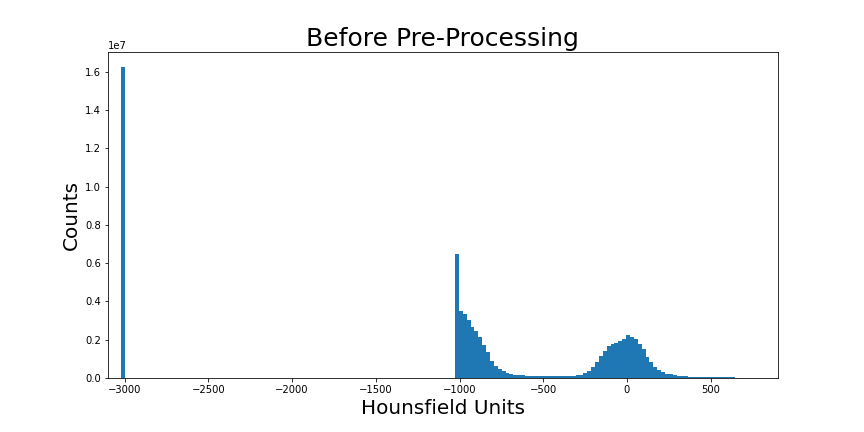
\includegraphics[scale=.4]{HU_before_rescaling.png}}
		%\hspace{1mm}
		\subfigure[Histogram of a CT scan after the registration]
		{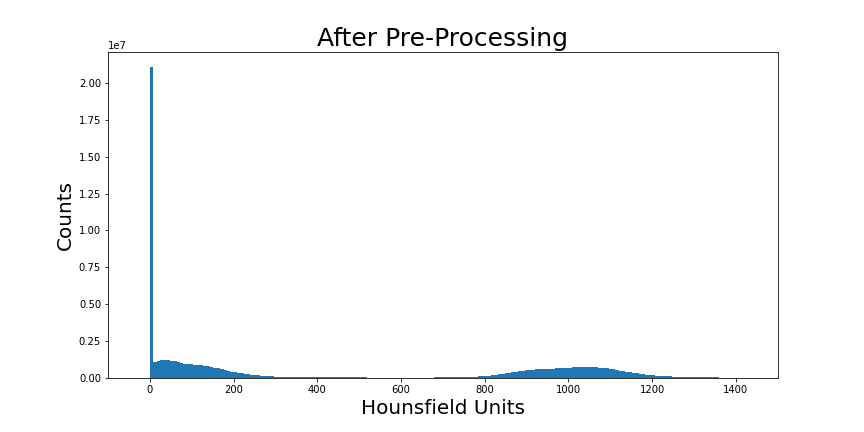
\includegraphics[scale=.4]{HU_after_rescaling.png}}
		\caption{Histogram of voxel values before and after the pre-processing. We can observe that before the pre processing there are some HU out of range, which are the values used to fill the regions outside the tube, and the air value is around $-1000\,HU$ according to HU definition. After the rescaling we can observe that all the values are non-negatives.}\label{fig:Pre-Processing}
	\end{figure}

	This step is not able to remove the airpokets and the motion artifacts, which we will see are the main source of error of this approach, so as future aim will be interesting to retrain this model in order to remove this kind of errors and improve the segmentation  quality.
	
	Now, we have found the mask for the lung regions, and we have managed the HU, so by a simple element wise multiplication we are able to isolate the lung from the rest of the body, removing also the organs, like heart and intestine, presents in the CT scans.\\
	
	This process, if no suitable GPU architecture(torch compatible), may be time expensive, requiring also more than 5 minutes for each scan, on the other hand, with a proper hardware configuration , will be very fast.\\
	
	Once lung regions are extracted, we are ready to perform the actual segmentation, or, if we haven't already estimate the centroids, performing the training step.\\
	
	
	\begin{algorithm}
		
		\SetAlgoLined
		\DontPrintSemicolon
		
		\KwData{CT scans volume}
		\KwResult{Volume with extracted lung}
		
		lung\_mask $\leftarrow$ create\_lung\_mask\;
		volume $\leftarrow$ (volume $<\,1200$) = volume air values\;
		volume $\leftarrow$ shift minimum to $1$\;
		lung $\leftarrow\,(volume\circ\,lung\_mask)$\;		
	\caption{Pseudo-code for the lung extraction script}	\label{alg:lungExtraction}
		
	\end{algorithm}
	
\end{document}